\section{Analysis}\label{sec:analysis}




\begin{figure}[!htb]
    \centering
    \begin{subfigure}{0.49\textwidth}
      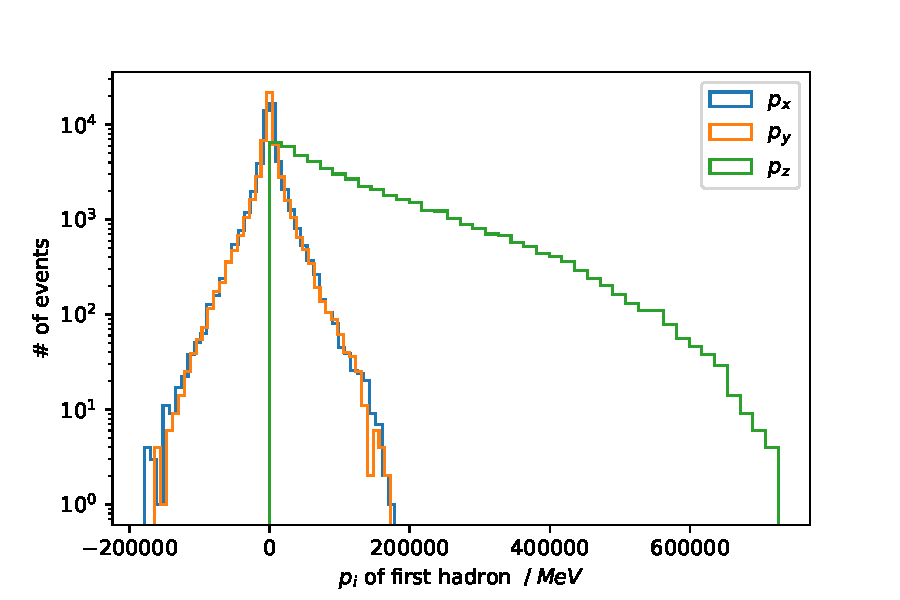
\includegraphics[width=\textwidth]{plots/momenta_H1_sim.pdf}
      \caption{Components of the 3-momentum of the first simulated hadron.}
      \label{fig:ProbPi}
    \end{subfigure}
    \begin{subfigure}{0.49\textwidth}
      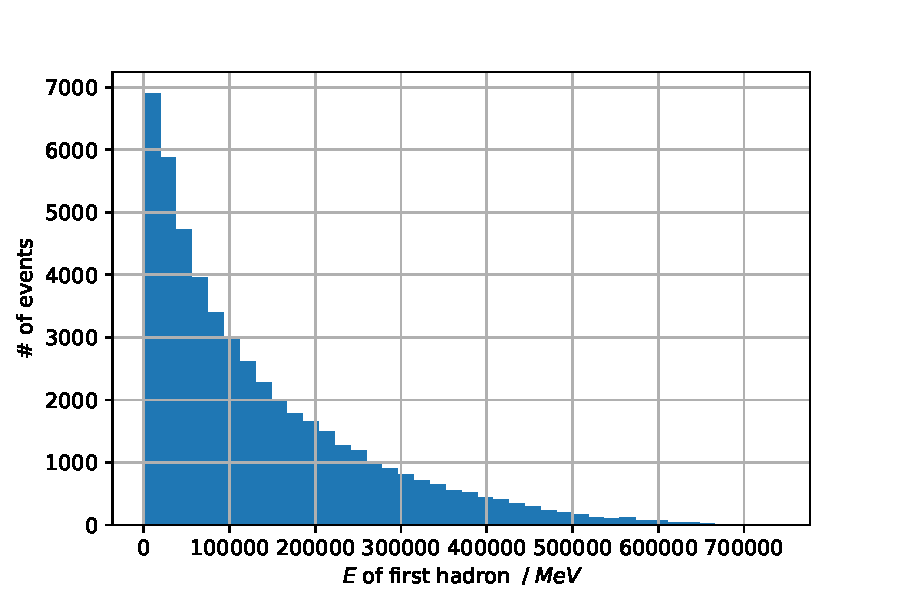
\includegraphics[width=\textwidth]{plots/energy_H1_sim.pdf}
      \caption{Energy of the first simulated hadron.}
      \label{fig:ProbK}
    \end{subfigure}
    \caption{Momentum components and energy of the first simulated hadron.}
    \end{figure}

\begin{figure}[!htb]
        \centering
        \begin{subfigure}{0.49\textwidth}
          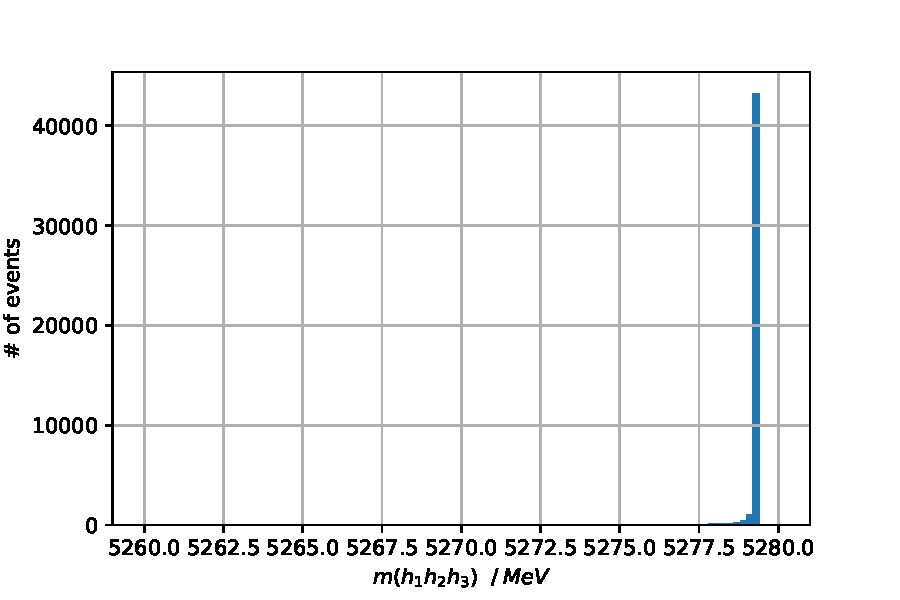
\includegraphics[width=\textwidth]{plots/mass_B_sim.pdf}
          \caption{Full spectrum of the invariant mass.}
          \label{fig:ProbPi}
        \end{subfigure}
        \begin{subfigure}{0.49\textwidth}
          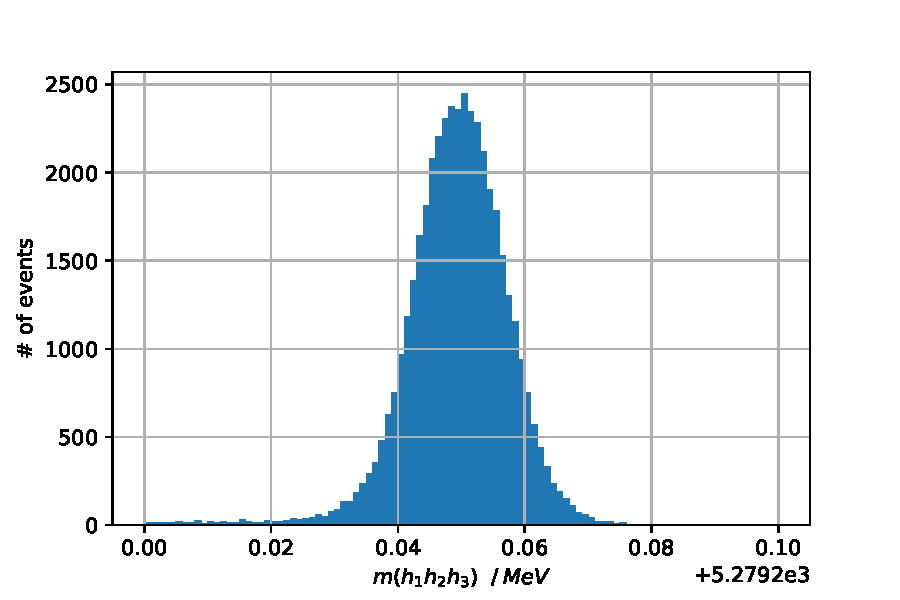
\includegraphics[width=\textwidth]{plots/masspeak_B_sim.pdf}
          \caption{Spectrum of the invariant mass restricted to $5279,2 \leq M \leq 5279,3$.}
          \label{fig:ProbK}
        \end{subfigure}
        \caption{Mass spectrum of the reconstructed B-mesons from simulated data.}
\end{figure}


\begin{figure}[!htb]
    \centering
    \begin{subfigure}{0.49\textwidth}
      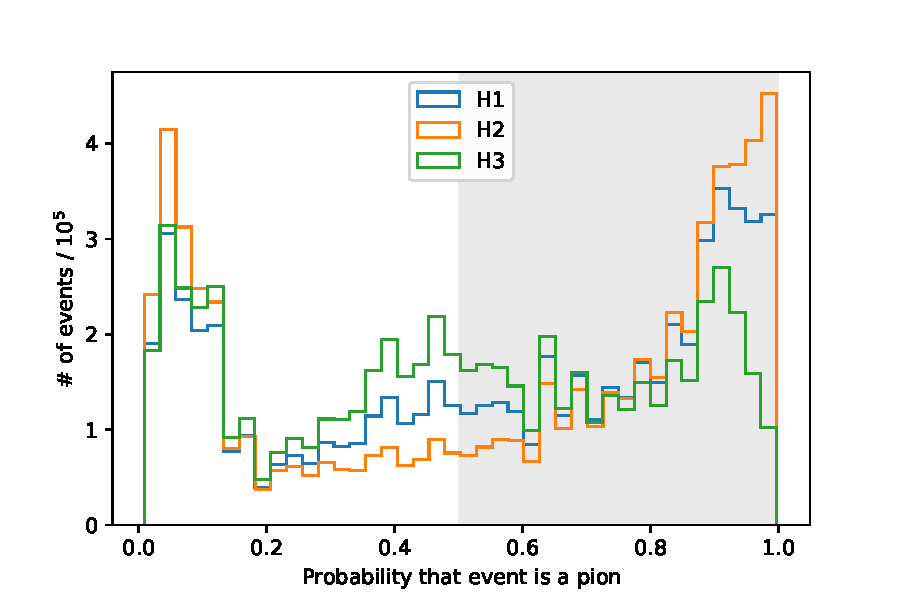
\includegraphics[width=\textwidth]{plots/ProbPi.pdf}
      \caption{Probability that the event is a pion.}
      \label{fig:ProbPi}
    \end{subfigure}
    \begin{subfigure}{0.49\textwidth}
      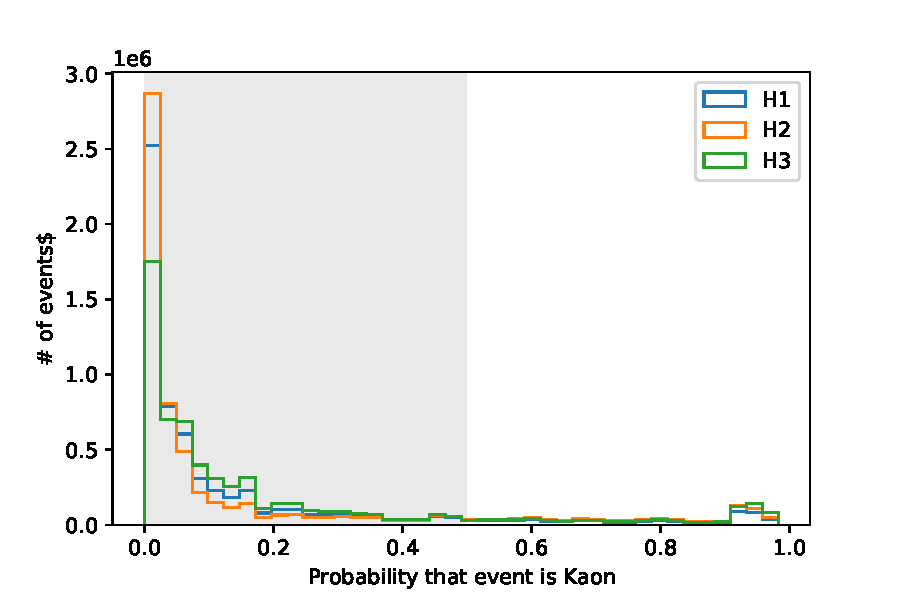
\includegraphics[width=\textwidth]{plots/ProbK.pdf}
      \caption{Probability that the event is a kaon.}
      \label{fig:ProbK}
    \end{subfigure}
    \caption{Probability spectrum that the measured hadron is either a pion or a kaon. 
    The area with the grey background is removed by the cut on the pion- and kaon-probability.}
\end{figure}

\begin{figure}[!htb]
    \centering
    \begin{subfigure}{0.49\textwidth}
      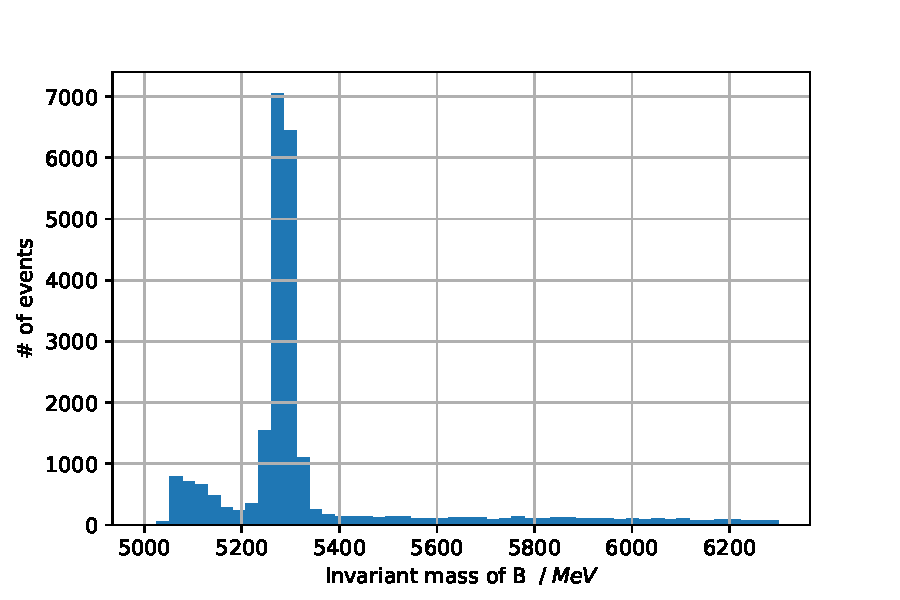
\includegraphics[width=\textwidth]{plots/mass_B.pdf}
      \caption{Full spectrum of the invariant mass.}
      \label{fig:ProbPi}
    \end{subfigure}
    \begin{subfigure}{0.49\textwidth}
      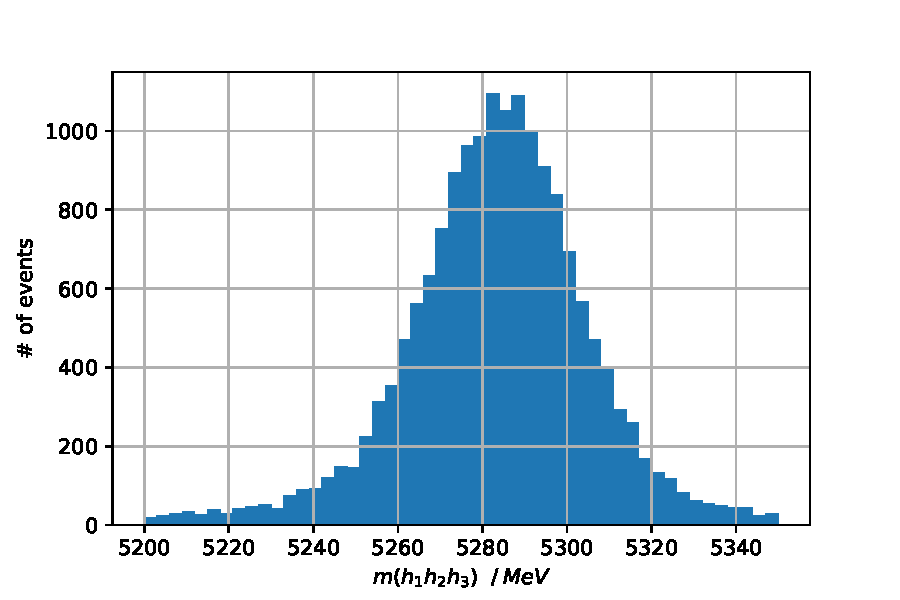
\includegraphics[width=\textwidth]{plots/masspeak_B.pdf}
      \caption{Spectrum of the invariant mass restricted to $5200 \leq M \leq 5350$.}
      \label{fig:ProbK}
    \end{subfigure}
    \caption{Mass spectrum of the B-mesons reconstructed from real data using the kaon mass hypothesis.}
\end{figure}


\begin{figure}[!htb]
  \centering
  \begin{subfigure}{0.49\textwidth}
    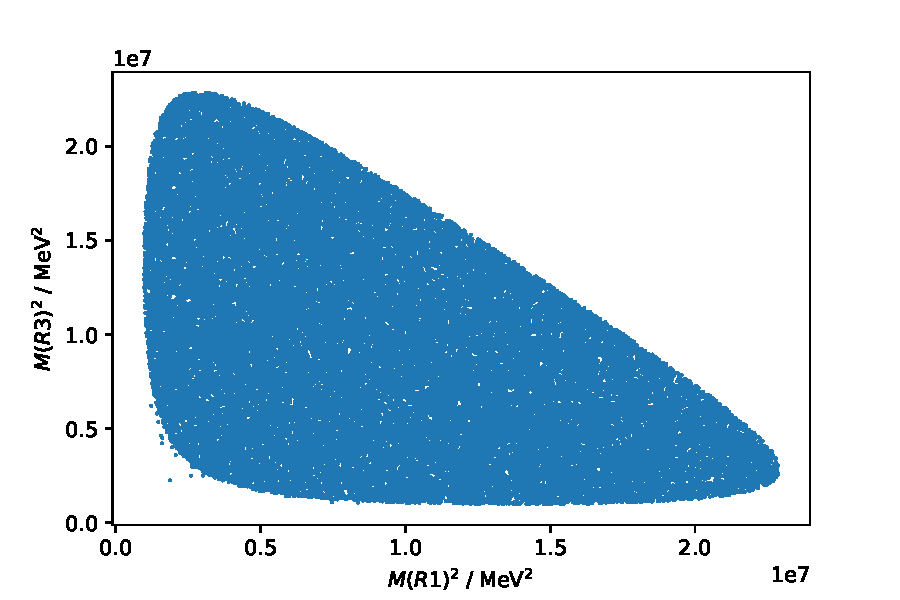
\includegraphics[width=\textwidth]{plots/Dalitz_sim_scatter.pdf}
    \caption{Scatterplot of the simulated data.}
    \label{fig:ProbPi}
  \end{subfigure}
  \begin{subfigure}{0.49\textwidth}
    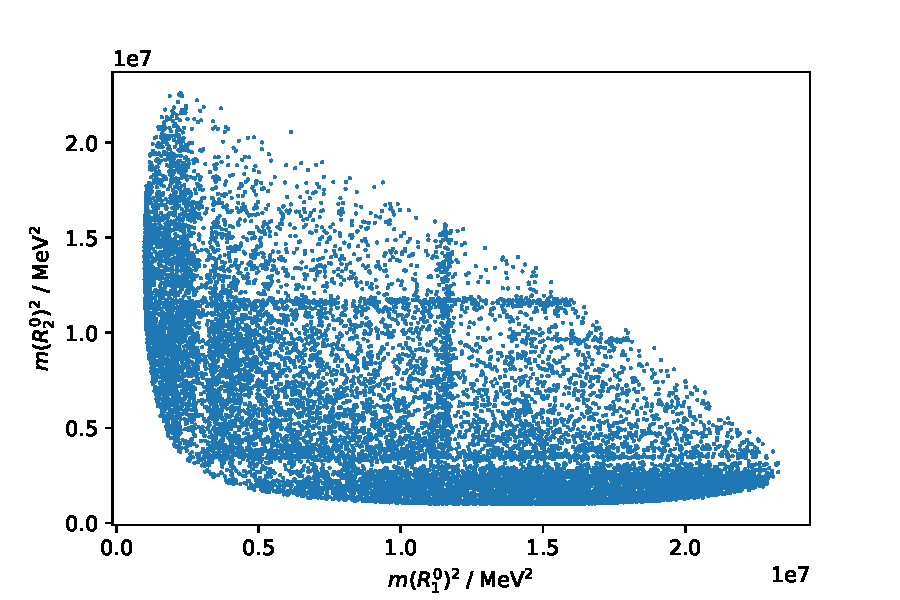
\includegraphics[width=\textwidth]{plots/Dalitz_scatter.pdf}
    \caption{Scatterplot of the real data.}
    \label{fig:ProbPi}
  \end{subfigure}
  \caption{Dalitz plots created from simulated and real data as a scatterplot}
\end{figure}


\begin{figure}[!htb]
  \centering
  \begin{subfigure}{0.49\textwidth}
    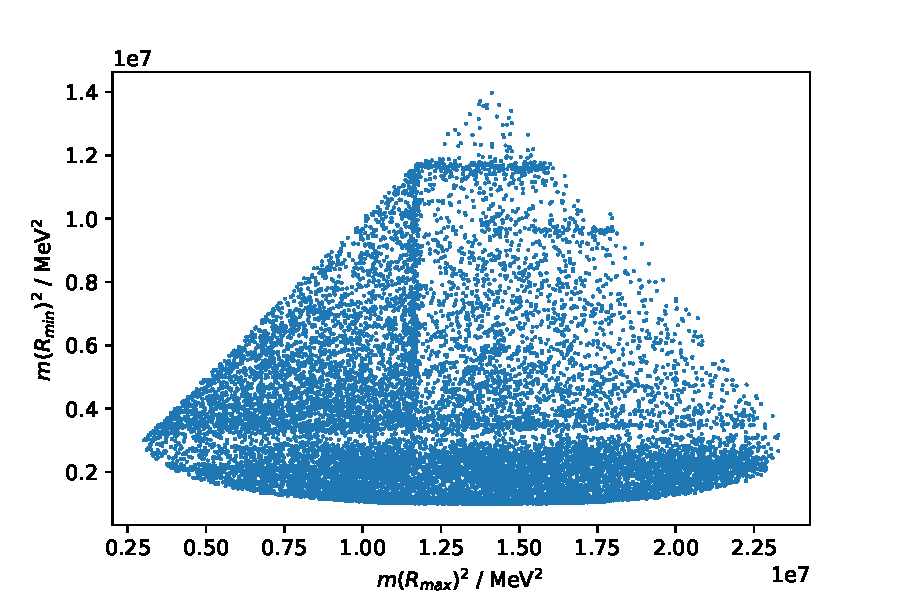
\includegraphics[width=\textwidth]{plots/Dalitz_sorted_scatter.pdf}
    \caption{Sorted Dalitz plot.}
    \label{fig:ProbPi}
  \end{subfigure}
  \begin{subfigure}{0.49\textwidth}
    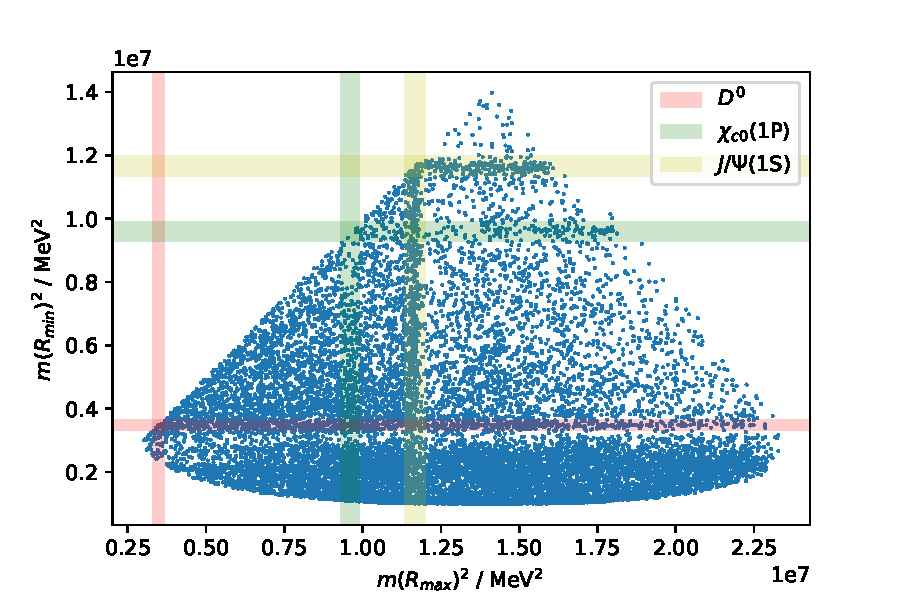
\includegraphics[width=\textwidth]{plots/Dalitz_sorted_scatter_band.pdf}
    \caption{Sorted Dalitz plot with events identified with resonance and removed by cuts marked by colored bands.}
    \label{fig:ProbPi}
  \end{subfigure}
  \begin{subfigure}{0.49\textwidth}
    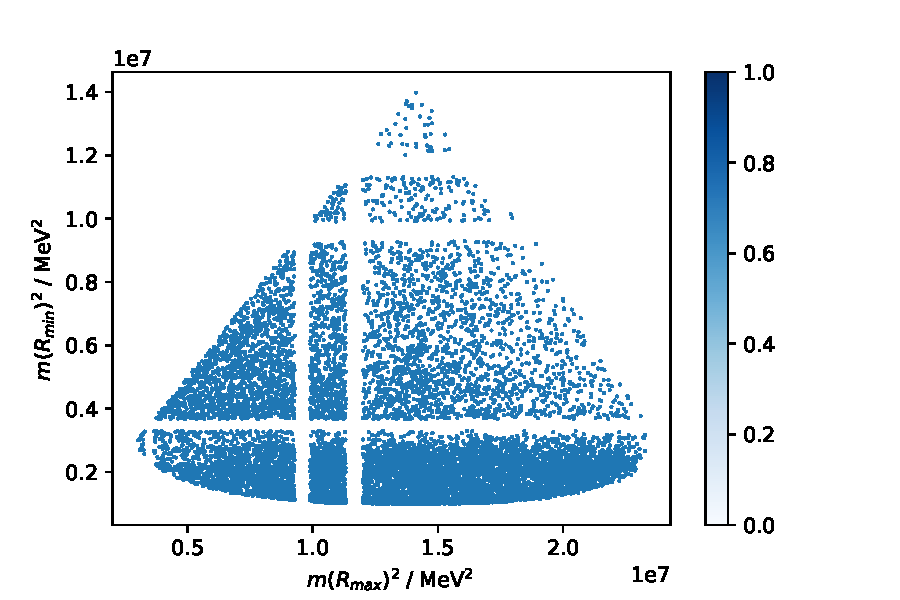
\includegraphics[width=\textwidth]{plots/Dalitz_sorted_scatter_cut.pdf}
    \caption{Sorted Dalitz plot after resonance cuts.}
    \label{fig:ProbPi}
  \end{subfigure}
  \caption{The sorted Dalitz plots created from the real data before and after the application of the cuts for the removal of the resonances.}
\end{figure}


\begin{figure}[!htb]
  \centering
  \begin{subfigure}{0.49\textwidth}
    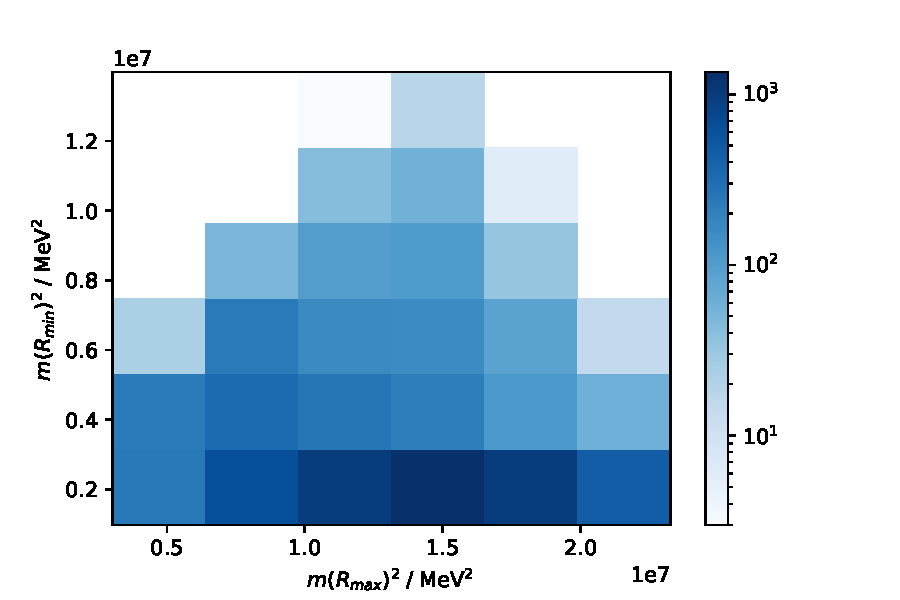
\includegraphics[width=\textwidth]{plots/Dalitz_sorted_bin_cut_bp.pdf}
    \caption{Binned histogram of the sorted Dalitz plot for the $B^+$-mesons.}
    \label{fig:ProbPi}
  \end{subfigure}
  \begin{subfigure}{0.49\textwidth}
    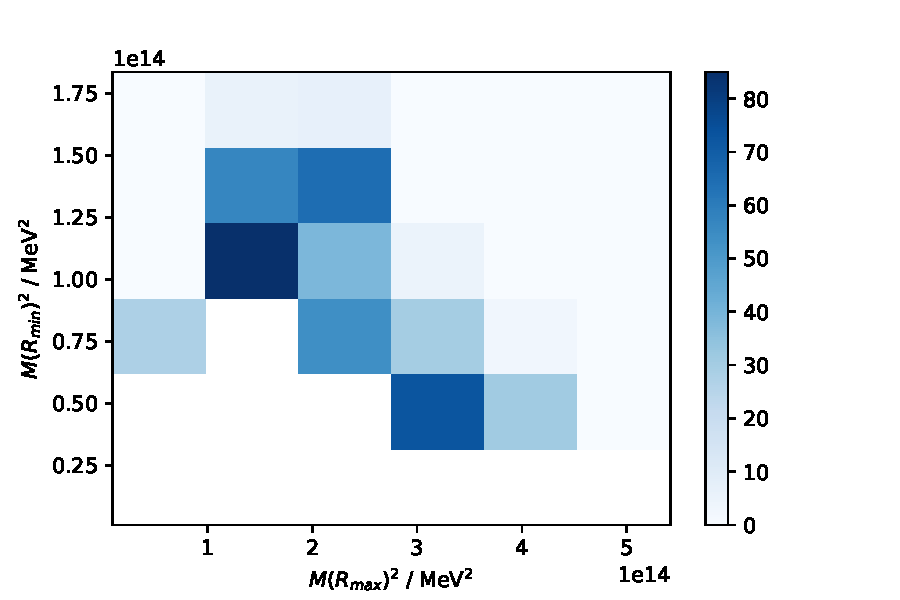
\includegraphics[width=\textwidth]{plots/Dalitz_sorted_bin_cut_bm.pdf}
    \caption{Binned histogram of the sorted Dalitz plot for the $B^-$-mesons.}
    \label{fig:ProbPi}
  \end{subfigure}
  \begin{subfigure}{0.49\textwidth}
    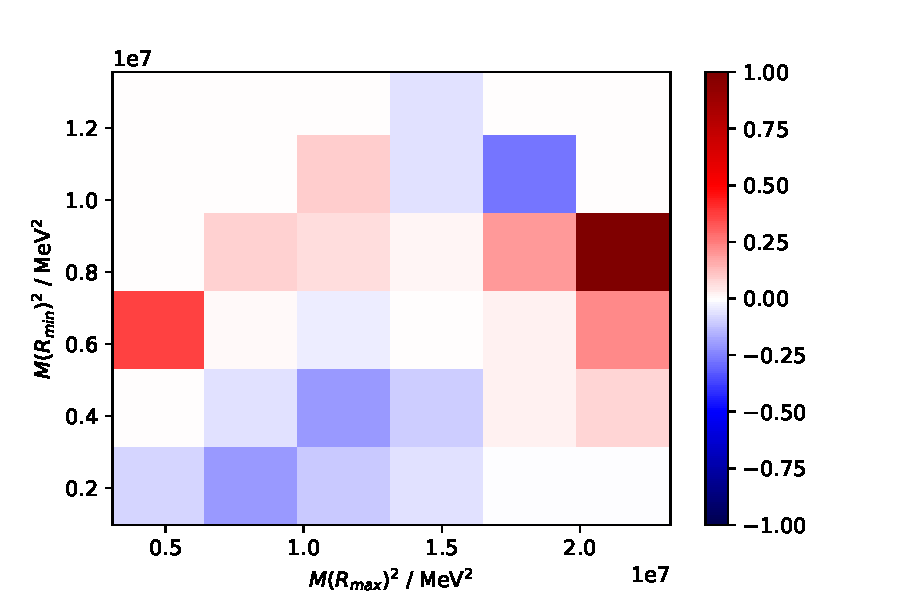
\includegraphics[width=\textwidth]{plots/Dalitz_sorted_Asym.pdf}
    \caption{The asymmetry calculated in each bin of the binned and sorted Dalitz plot.}
    \label{fig:ProbPi}
  \end{subfigure}
  \begin{subfigure}{0.49\textwidth}
    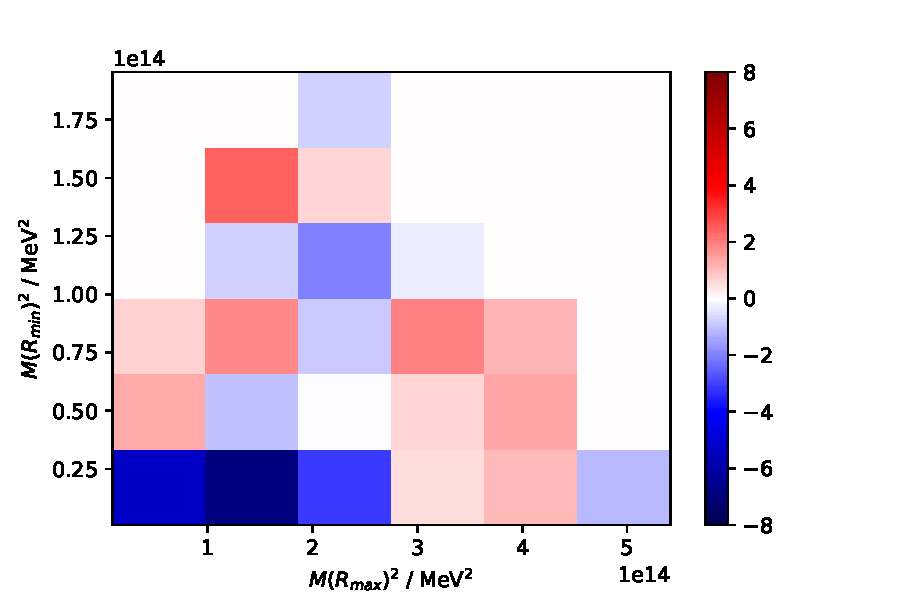
\includegraphics[width=\textwidth]{plots/Dalitz_sorted_bin_cut_sig.pdf}
    \caption{The significance calculated in each bin of the binned and sorted Dalitz plot.}
    \label{fig:ProbPi}
  \end{subfigure}
  \caption{The binned sorted Dalitz plots determined for the $B^+$- and $B^-$-mesons and the significance and asymmetry calculated in each bin after the application 
  of all cuts.}
\end{figure}


\begin{figure}[!htb]
  \centering
    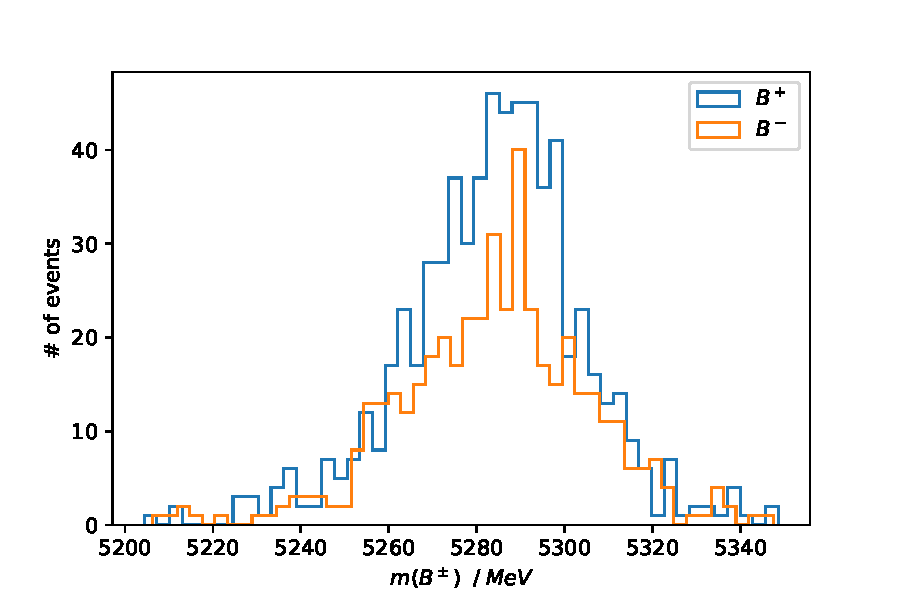
\includegraphics[width=\textwidth]{plots/num_b.pdf}
  \caption{The number of reconstructed $B^+$- and $B^-$-mesons in the bin 
  $0,97 \cdot 10^{14} \, \si{\mega\eV\squared} \lesssim M(R_\text{max})^2 \lesssim 1,86 \cdot 10^{14} \, \si{\mega\eV\squared}$ and 
  $0.01 \cdot 10^{14} \, \si{\mega\eV\squared} \lesssim M(R_\text{max})^2 \lesssim 0,33 \cdot 10^{14} \, \si{\mega\eV\squared}$.}
\end{figure}


